\documentclass{beamer}
\usepackage{ctex, hyperref}
\usepackage[T1]{fontenc}

% other packages
\usepackage{latexsym,amsmath,xcolor,multicol,booktabs,calligra}
\usepackage{graphicx,pstricks,listings,stackengine}
\usepackage[normalem]{ulem}

\author{userElaina}
\title{Deep learning from crowds}
\institute{School of AI}
\date{2024.08.26}
\usepackage{JilinUniv}

\def\cmd#1{\texttt{\color{red}\footnotesize $\backslash$#1}}
\def\env#1{\texttt{\color{blue}\footnotesize #1}}
\definecolor{deepblue}{rgb}{0,0,0.5}
\definecolor{deepred}{rgb}{0.6,0,0}
\definecolor{deepgreen}{rgb}{0,0.5,0}
\definecolor{halfgray}{gray}{0.55}

\lstset{
    basicstyle=\ttfamily\small,
    keywordstyle=\bfseries\color{deepblue},
    emphstyle=\ttfamily\color{deepred},    % Custom highlighting style
    stringstyle=\color{deepgreen},
    numbers=left,
    numberstyle=\small\color{halfgray},
    rulesepcolor=\color{red!20!green!20!blue!20},
    frame=shadowbox,
}

\begin{document}

\kaishu
\begin{frame}
    \titlepage
    \begin{figure}[htpb]
        \begin{center}
            
\includegraphics[width=0.15\linewidth]{pic/Jilin_University_Logo.eps}
        \end{center}
    \end{figure}
\end{frame}

% \begin{frame}
% \tableofcontents[sectionstyle=show,subsectionstyle=show/shaded/hide,subsubsectionstyle=show/shaded/hide]
% \end{frame}

\section{Deep learning from crowds}

\begin{frame}{Architecture}
    \begin{figure}[c]
        \centering
        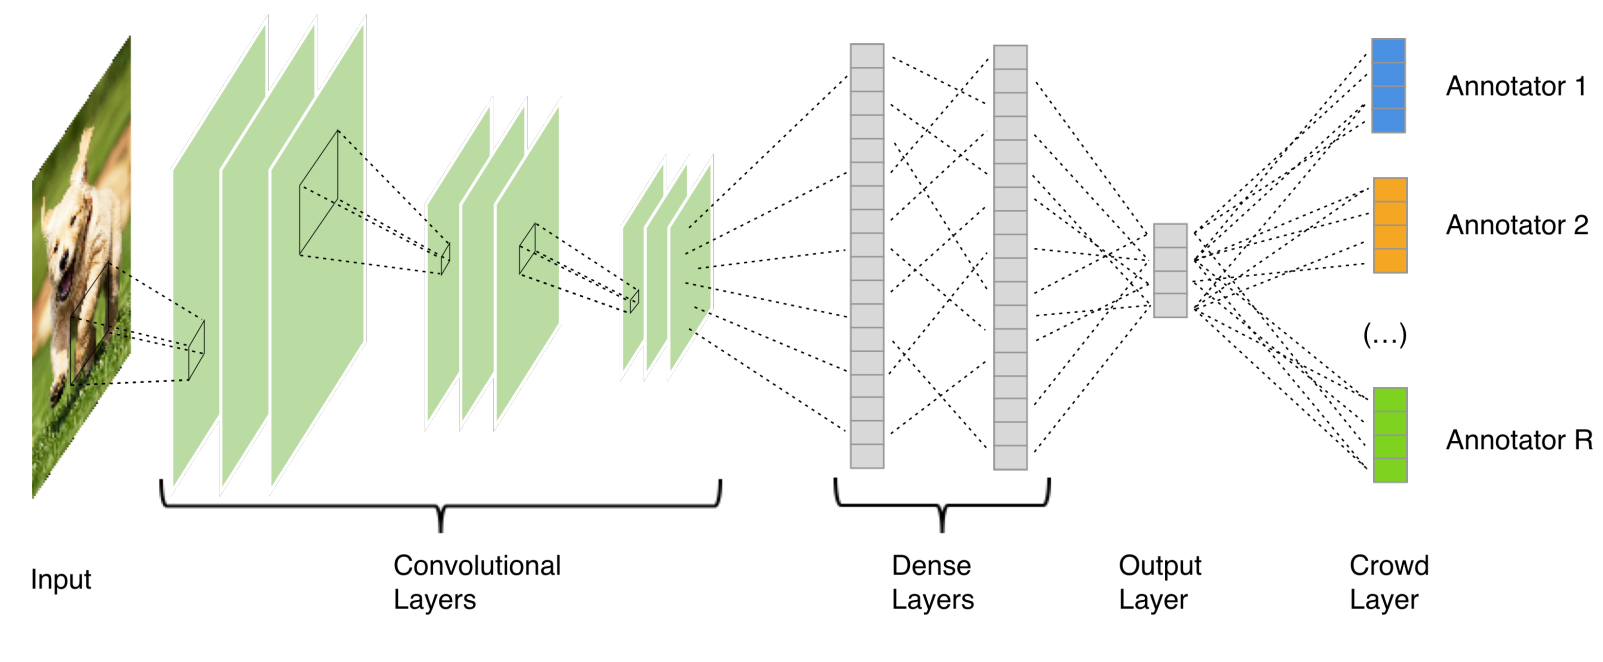
\includegraphics[width=\textwidth]{pic/8.png}
        \caption{Classification with R annotators}
    \end{figure}
\end{frame}

\begin{frame}{Notice}
    \begin{itemize}
        \item $C$ number of classes
        \item $R$ number of annotators
        \item $\sigma = \{\sigma_1, ..., \sigma_C\}$ the output of DNN
        \item $y_r$ actual label
        \item $f_r$ annotator-specific function
        \item $a_r = f_r(\sigma) = W_r \sigma$
        \item $o_{r,c} = \frac{e^{a_{r,c}}}{\sum_{j=1}^C e^{a_{r,j}}}$ the output of the crowd layer
    \end{itemize}
\end{frame}

\begin{frame}{Backward (Crowd Layer)}
    \begin{align*}
        E
        &= \sum_{r=1}^R E_r(o_r,y_r)\\
        \textcolor{red}{\frac{\partial E}{\partial \sigma}}
        &= \sum_{r=1}^R \frac{\partial E_r(o_r,y_r)}{\partial \sigma} \\
        &= \sum_{r=1}^R W_r \frac{\partial E}{\partial a_r}
    \end{align*}
\end{frame}

\begin{frame}{Notice}
    \begin{itemize}
        \item $\sigma = \{\sigma_1, ..., \sigma_C\}$ the output of DNN (layer -1)
        \item $g$ activation function
        \item $\theta$ thresholds of layer -1
        \item $\beta = \{\beta_1, ..., \beta_C\}$ input for layer -1
        \item $\delta = \{\delta_i | i\}$ output of layer -2
        \item $w = \{w_{i,c} | i,c\}$ weights between layers -1 and -2
    \end{itemize}
\end{frame}

\begin{frame}{Backward (Linear Layer)}
    \begin{align*}
        \sigma_c &= g(\beta_c-\theta_c) \\
        \beta_c &= \sum_i w_{i,c}\delta_i \\
        \frac{\partial E}{\partial w_{i,c}}
        &= \textcolor{red}{\frac{\partial E}{\partial\sigma_c}}\frac{\partial\sigma_c}{\partial\beta_c}\frac{\partial\beta_c}{\partial w_{i,c}} \\
        &= \textcolor{red}{\frac{\partial E}{\partial\sigma_c}}g'(\beta_c-\theta_c)\delta_i
    \end{align*}
\end{frame}

\begin{frame}{parameters to be optimized}
    \begin{itemize}
        \item parameters of DNN ($w, \theta, ...$)
        \item $W^r$
    \end{itemize}
\end{frame}

\end{document}

% Q model para
